%%%%%%%%%%%%%%%%%%%%%%%%%%%%%%%%%%%%%%%%%
% Short Sectioned Assignment LaTeX Template Version 1.0 (5/5/12)
% This template has been downloaded from: http://www.LaTeXTemplates.com
% Original author:  Frits Wenneker (http://www.howtotex.com)
% License: CC BY-NC-SA 3.0 (http://creativecommons.org/licenses/by-nc-sa/3.0/)
%%%%%%%%%%%%%%%%%%%%%%%%%%%%%%%%%%%%%%%%%

%----------------------------------------------------------------------------------------
%	PACKAGES AND OTHER DOCUMENT CONFIGURATIONS
%----------------------------------------------------------------------------------------

\documentclass[paper=a4, fontsize=11pt]{scrartcl} % A4 paper and 11pt font size

% ---- Entrada y salida de texto -----

\usepackage[T1]{fontenc} % Use 8-bit encoding that has 256 glyphs
\usepackage[utf8]{inputenc}
%\usepackage{fourier} % Use the Adobe Utopia font for the document - comment this line to return to the LaTeX default
\usepackage{hyperref}
\usepackage{enumitem} 
% ---- Idioma --------

\usepackage[spanish, es-tabla]{babel} % Selecciona el español para palabras introducidas automáticamente, p.ej. "septiembre" en la fecha y especifica que se use la palabra Tabla en vez de Cuadro

% ---- Otros paquetes ----

\usepackage{amsmath,amsfonts,amsthm} % Math packages
%\usepackage{graphics,graphicx, floatrow} %para incluir imágenes y notas en las imágenes
\usepackage{graphics,graphicx, float} %para incluir imágenes y colocarlas

% Para hacer tablas comlejas
%\usepackage{multirow}
%\usepackage{threeparttable}

%\usepackage{sectsty} % Allows customizing section commands
%\allsectionsfont{\centering \normalfont\scshape} % Make all sections centered, the default font and small caps

\usepackage{fancyhdr} % Custom headers and footers
\pagestyle{fancyplain} % Makes all pages in the document conform to the custom headers and footers
\fancyhead{} % No page header - if you want one, create it in the same way as the footers below
\fancyfoot[L]{} % Empty left footer
\fancyfoot[C]{} % Empty center footer
\fancyfoot[R]{\thepage} % Page numbering for right footer
\renewcommand{\headrulewidth}{0pt} % Remove header underlines
\renewcommand{\footrulewidth}{0pt} % Remove footer underlines
\setlength{\headheight}{13.6pt} % Customize the height of the header

\numberwithin{equation}{section} % Number equations within sections (i.e. 1.1, 1.2, 2.1, 2.2 instead of 1, 2, 3, 4)
\numberwithin{figure}{section} % Number figures within sections (i.e. 1.1, 1.2, 2.1, 2.2 instead of 1, 2, 3, 4)
\numberwithin{table}{section} % Number tables within sections (i.e. 1.1, 1.2, 2.1, 2.2 instead of 1, 2, 3, 4)

\setlength\parindent{0pt} % Removes all indentation from paragraphs - comment this line for an assignment with lots of text

\newcommand{\horrule}[1]{\rule{\linewidth}{#1}} % Create horizontal rule command with 1 argument of height


%----------------------------------------------------------------------------------------
%	TÍTULO Y DATOS DEL ALUMNO
%----------------------------------------------------------------------------------------
\sffamily


\title{	
\normalfont \normalsize 
\textsc{{\bf Recuperación de Información (2016-2017)} \\ Grado en Ingeniería Informática \\ Universidad de Granada} \\ [25pt] % Your university, school and/or department name(s)
\horrule{0.5pt} \\[0.4cm] % Thin top horizontal rule
\huge Memoria Práctica Lucene \\ % The assignment title
\horrule{2pt} \\[0.5cm] % Thick bottom horizontal rule
}

\author{Pablo Martínez Ruano} % Nombre y apellidos

\date{\normalsize\today} % Incluye la fecha actual

%----------------------------------------------------------------------------------------
% DOCUMENTO
%----------------------------------------------------------------------------------------

\usepackage{url}
\usepackage{hyperref}
\usepackage{csquotes}
\usepackage{listings}


\begin{document}

\maketitle % Muestra el Título

\newpage %inserta un salto de página

\tableofcontents % para generar el índice de contenidos

\listoffigures

\listoftables

\newpage

\section{Introducción}
A continuación se encuentra la documentación asociada a la práctica desarrollada en la asignatura RI, en la cual vamos a llevar a cabo el desarrollo de un sistema de recuperación de información.Nuestro proyecto consiste en desarrollar una aplicación de recuperación de información usando Lucene. A lo largo de este proceso obtendremos las siguientes competencias:
\begin{enumerate}

  \item Adquirir las destrezas, conocimientos y técnicas básicas para buscar información textual.
  \item Entender el concepto de modelo de recuperación de información
  \item Adquirir una visión general del proceso de recuperación de información. 
  \item Conocer los diferente componentes de un sistema de recuperación de información, su funcionamiento y relaciones entre ellos. 
  \item Comprender las peculiaridades de la recuperación de información XML y las similitudes y diferencias con la recuperación de información de la informática clásica.
  \item Identificar los elementos que conforman la Web, así como conocer la estructura.
  \item Conocer las técnicas específicas para la recuperación de información en la Web.
  \item Asumir la importancia de la recuperación de información en e diseño y desarrollo de sistemas de información.
  \item Analizar problemas de acceso de información en el marco de los sistemas de información y diseñar un sistema de recuperación de información que les de solución.
  \item Ser capaz de integrar un sistema de recuperación de información en un sistema de información.
  \item Conocer las instituciones responsables de la legislación vigente en el ámbito de los sistemas de información y ser conscientes de la normativa aplicable en cada momento. Así como poder evaluar la adecuación de un sistema de información a la normativa y legislación vigente. 

\end{enumerate}

\section{Nuestro Proyecto}
Nuestro proyecto va a ser una aplicación de recuperación de información para twitter. La idea es sencilla, nuestra aplicación estara formada por 2 ventanas. En una ventana estara compuesta por por un buscador. En la misma ventana y para usar el buscador tendremos a disposición un menu de opciones de aquello que deseamos filtrar en la busqueda. También como extra disponemos de un boton para imprimir el contenido en un fichero de texto.

\begin{figure}[H] %con el [H] le obligamos a situar aquí la figura
\centering
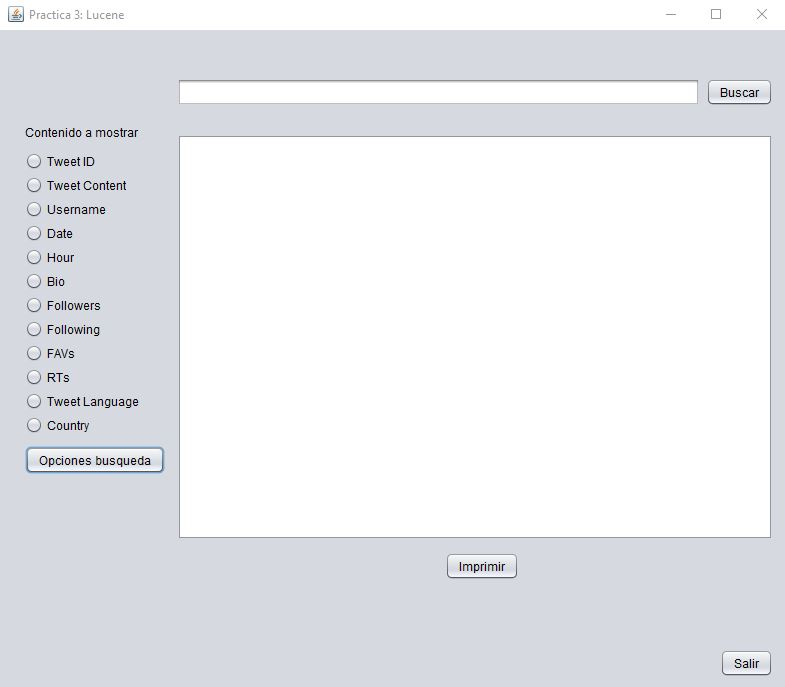
\includegraphics[trim={0cm 0 0 0},clip,scale=0.8]{/home/pablo/Descargas/P2-LuisGilGui/RI/Captura2.JPG}  %el parámetro scale permite agrandar o achicar la imagen. En el nombre de archivo puede especificar directorios
\caption{Muestra de la interfaz gráfica principal.}\label{figura1}
\end{figure}

También disponemos de una segunda ventana, esta será emergente nos mostrara un menú de aquello que desemos buscar.

\begin{figure}[H] %con el [H] le obligamos a situar aquí la figura
\centering
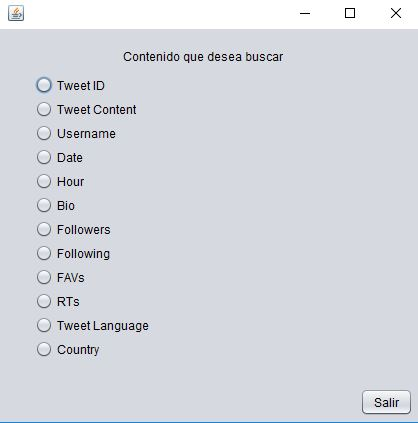
\includegraphics[trim={0cm 0 0 0},clip,scale=0.9]{/home/pablo/Descargas/P2-LuisGilGui/RI/Captura.JPG}  %el parámetro scale permite agrandar o achicar la imagen. En el nombre de archivo puede especificar directorios
\caption{Ventana emergente de nuestra interfaz gráfica}\label{figura1}
\end{figure}

El modo de uso es bastante sencillo, vamos explicarlo con un ejemplo. Imaginemos que insertamos en el buscador "2000" y en opciones de busqueda marcamos Tweet Content. Es hara buscar tweet que contenga el numero 2000. Esto es solamente para buscar, para mostrar la información en opciones vamos a suponer que marcamos Nickname, Tweet Content, FAVs y RTs. Esto hara que buscara los contenido del tweet que tenga el numero 2000, pero mostrara el nickname del autor del tweet, el contenido del tweet, sus favs y rts.

\section{Análisis previo de requisitos}

A continuación vamos a comentar el análisis previo de requisitos que hemos realizado para el proyecto, para ello vamos hablar de los elementos funciones y de los elementos no funcionales.


\subsection{Funcionales}
RF1.\textbf{BuscarTUsername}El usuario usa el sistema de recuperación de información para buscar el Username\\

RF2\textbf{BuscarNickname.}El usuario usa el sistema de recuperación de información para buscar el Nickname \\

RF3.\textbf{BuscarTweetContent.}El usuario usa el sistema de recuperación de información para buscar el contenido del tweet\\

RF4.\textbf{BuscarDate.}El usuario usa el sistema de recuperación de información para buscar la fecha del tweet\\

RF5.\textbf{BuscarBio.}El usuario usa el sistema de recuperación de información para buscar las biograficas de los usuarios.\\

RF6.\textbf{BuscarCountry.}El usuario usa el sistema de recuperación de información para buscar el pais del usuario.\\

RF7.\textbf{BuscarPlace.}El usuario usa el sistema de recuperación de información para buscar el lugar donde se escribio el tweet\\

RF8.\textbf{BuscarLanguage.}El usuario usa el sistema de recuperación de información para buscar el lenguaje\\

RF9.\textbf{BuscarFAVs.}El usuario usa el sistema de recuperación de información para buscar los Favs\\

RF10.\textbf{BuscarRTs.}El usuario usa el sistema de recuperación de información para buscar los RTs\\

RF11.\textbf{FiltrarTUsername}El usuario usa el sistema de recuperación de información para filtrar el Username\\

RF12\textbf{FiltrarNickname.}El usuario usa el sistema de recuperación de información para filtrar el Nickname\\

RF13.\textbf{FiltrarTweetContent.}El usuario usa el sistema de recuperación de información para filtrar el contenido del tweet\\

RF14.\textbf{FiltrarDate.}El usuario usa el sistema de recuperación de información para filtrar la fecha\\

RF15.\textbf{FiltrarBio.}El usuario usa el sistema de recuperación de información para filtrar la biografia del usuario.\\

RF16.\textbf{FiltrarCountry.}El usuario usa el sistema de recuperación de información para filtrar el pais\\

RF17.\textbf{FiltrarPlace.}El usuario usa el sistema de recuperación de información para filtrar el lugar\\

RF18.\textbf{FiltrarLanguage.}El usuario usa el sistema de recuperación de información para filtrar el idioma\\

RF19.\textbf{FiltrarFAVs.}El usuario usa el sistema de recuperación de información para filtrar los FAVs\\

RF20.\textbf{FiltrarRTs.}El usuario usa el sistema de recuperación de información para filtrar los RTs\\


\subsection{No funcionales}

\textbf{RNF1.}El sistema no deberá mostrar nada si no se marcado en los menus ninguna opción.
\textbf{RNF2.}Las búsquedas simultaneas solo se podran realizar las que se hayan descrito en el manual.
\textbf{RNF3.}El cuadro de texto se debera mover tanto largo como ancho para mostrar el contenido completo.
\textbf{RNF4.}Se debe incluir una funcion para imprimir los resultados y de esa manera guardarlos.
\textbf{RNF5.}Los ficheros que indexaremos seran formato .csv.

\section{Diseño de la solución}

Ahora vamos comentar el diseño que vamos enfocar para dar solución a nuestro problema. Para ello vamos comentar la arquitectura de nuestro problema, los posibles escenarios, la vista de procesos y la vista de desarrollo.

\subsection{Arquitectura de nuestro programa}

Para llegar a cabo este proyecto no necesitamos un hardware costoso, nos vale con nuestro ordenador personal. El sistema operativo a utilizar también es indiferente, nos sirve tanto Windows, MAC OS o algún Linux ya que vamos utilizar la máquina virtual de Java para ejecutar la aplicación, el unico requisito es que nuestro SO soporte Java. Lo que si necesitamos es tener las biblitecas de Lucene y Tika , que son las bibliotecas que vamos utilizar para llevar acabo el proyecto.

\begin{figure}[H] %con el [H] le obligamos a situar aquí la figura
\centering
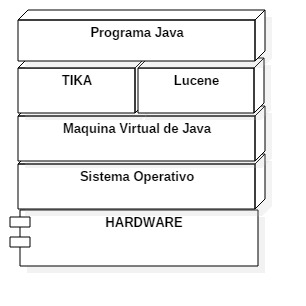
\includegraphics[trim={0cm 0 0 0},clip,scale=0.8]{/home/pablo/Descargas/P2-LuisGilGui/RI/PhysicalView.jpg}  %el parámetro scale permite agrandar o achicar la imagen. En el nombre de archivo puede especificar directorios
\caption{Muestra de la interfaz gráfica principal.}\label{figura1}
\end{figure}
\subsection{Escenario}

A continuación hemos preparado un esquema sobre el escenario posible de interacción de los usuarios con el software.

\begin{figure}[H] %con el [H] le obligamos a situar aquí la figura
\centering
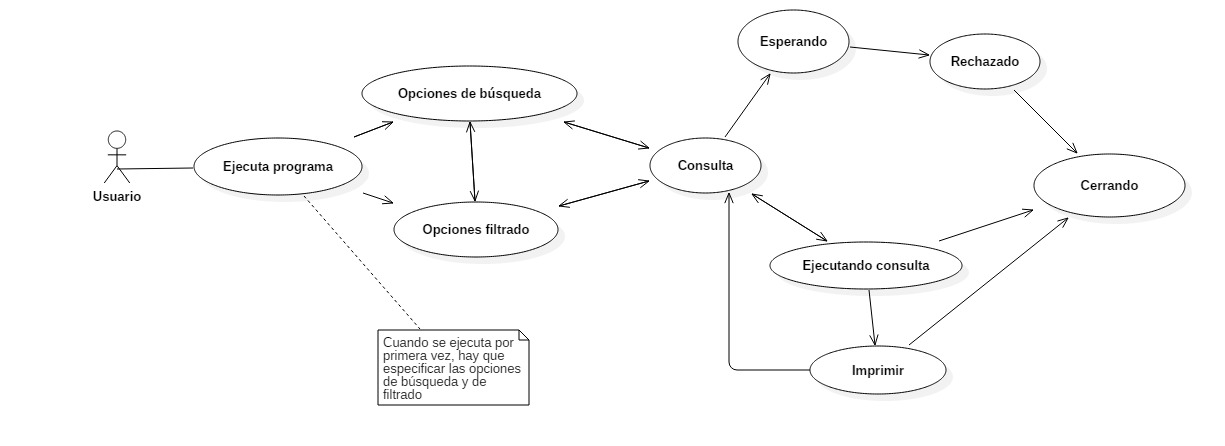
\includegraphics[trim={0cm 0 0 0},clip,scale=0.4]{/home/pablo/Descargas/P2-LuisGilGui/RI/Scenarios.jpg}  %el parámetro scale permite agrandar o achicar la imagen. En el nombre de archivo puede especificar directorios
\caption{Muestra de la interfaz gráfica principal.}\label{figura1}
\end{figure}

Como se puede ver no es muy complejo, una vez se haya iniciado el programa el usuario por primera vez tendra que marcar lo que desea buscar y filtrar, una vez realizado esto el usuario interacciona con el buscador. Pueden darse 2 casos: Que la buscado no de resultado lo cual provoca el cierre el programa en caso de error, o que sastifaga su busqueda. Si satisface su busqueda se le da la opcion de imprimir para guardar su búsqueda y después el usuario puede realizar otra busqueda o usar el programa.
\subsection{Vista de los procesos}

Ahora vamos a mostrar una vista de los procesos, en cual de forma sencilla vamos a mostrar de manera gráfica todo el abanico de opciones que proporciona nuestro software, como ya antes habiamos especificados en nuestros requisitos funcionales

\begin{figure}[H] %con el [H] le obligamos a situar aquí la figura
\centering
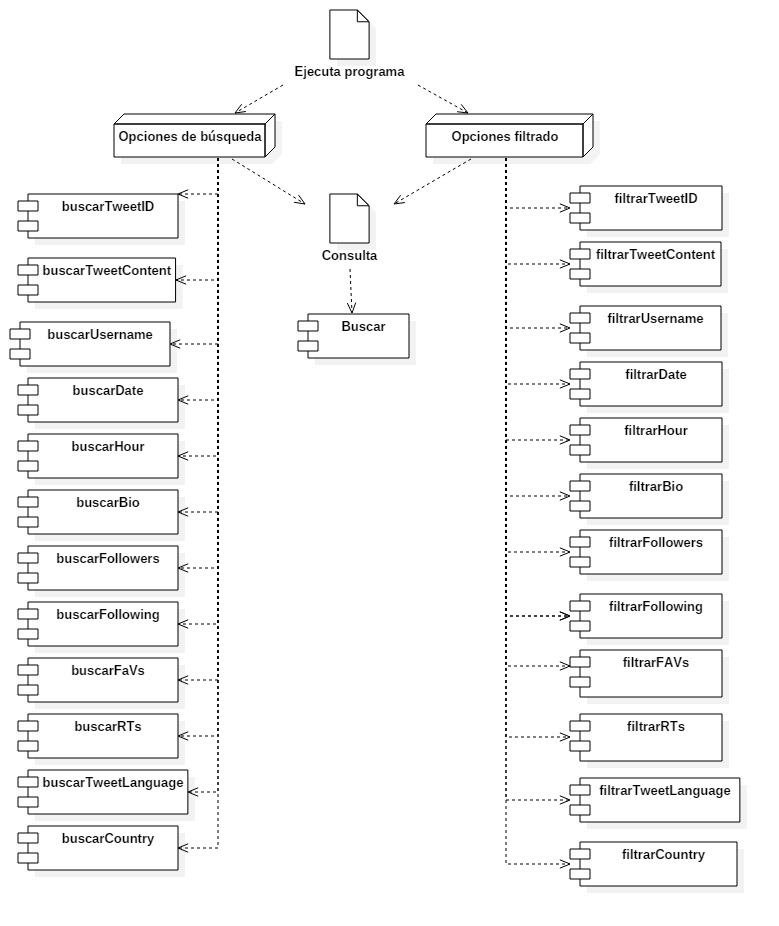
\includegraphics[trim={0cm 0 0 0},clip,scale=0.5]{/home/pablo/Descargas/P2-LuisGilGui/RI/ProcessView.jpg}  %el parámetro scale permite agrandar o achicar la imagen. En el nombre de archivo puede especificar directorios
\caption{Muestra de la interfaz gráfica principal.}\label{figura1}
\end{figure}
\subsection{Vista del desarrollo}
\begin{figure}[H] %con el [H] le obligamos a situar aquí la figura
\centering
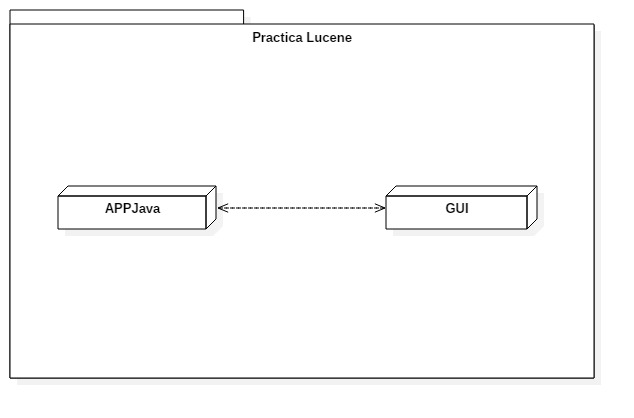
\includegraphics[trim={0cm 0 0 0},clip,scale=0.8]{/home/pablo/Descargas/P2-LuisGilGui/RI/DevelopmentView.jpg}  %el parámetro scale permite agrandar o achicar la imagen. En el nombre de archivo puede especificar directorios
\caption{Muestra de la interfaz gráfica principal.}\label{figura1}
\end{figure}

\section{Codigo}
\subsection{Indexar}
\lstset{breaklines=true}
\lstinputlisting[language=Java]{/home/pablo/Descargas/P2-LuisGilGui/codigo/Indexacion.java}
\subsection{Buscar}
\lstinputlisting[language=Java]{/home/pablo/Descargas/P2-LuisGilGui/codigo/Busqueda.java}
\section{Manual de Usuario}


%------------------------------------------------

\bibliography{citas} %archivo citas.bib que contiene las entradas 
\bibliographystyle{plain} % hay varias formas de citar



\end{document}

